\documentclass[12pt]{article}
\renewcommand{\baselinestretch}{0.95}

\usepackage{sbc-template}
\usepackage{graphicx,url}
\usepackage[utf8]{inputenc}
\makeatletter\let\normalsfcodes\relax\makeatother
\usepackage[brazil]{babel}
\AtBeginDocument{\providecommand{\normalsfcodes}{}}
\usepackage{booktabs}
\usepackage{tabularx}
\usepackage{longtable}
\usepackage{tikz}
\usepackage{amsmath}
\usepackage{amssymb}
\usepackage{enumitem}
\usepackage[table]{xcolor}
\usepackage{multirow}
\usepackage{pgfgantt}
\usepackage{pgfplots}
\pgfplotsset{compat=1.17}
\usepackage[most]{tcolorbox}
\usepackage{listings}
\usepackage{caption}
\usetikzlibrary{arrows.meta, positioning, shapes.geometric, fit, backgrounds, calc}
\makeatletter
\providecommand\normalsfcodes{%
  \sfcode`\.=\@m
  \sfcode`\?=\@m
  \sfcode`\!=\@m
  \sfcode`\:=\@m
  \sfcode`\;=\@m
}
\makeatother

\newcommand{\code}[1]{\texttt{#1}}
\newcommand{\proj}{AI-CogWalk-NAV}
\def\UrlBreaks{\do\/\do-\do_}
\newcolumntype{Y}{>{\raggedright\arraybackslash}X}
\newcommand{\Ph}{P_H}
\newcommand{\Pp}{\hat{P}}
\DeclareMathOperator{\JSD}{JSD}

% Caixas de status: o que é resultado real e o que é planejado
\newtcolorbox{real}{colback=green!4,colframe=green!45!black,boxrule=0.5pt,arc=2pt,left=4pt,right=4pt,top=2pt,bottom=2pt,
  fonttitle=\bfseries\small,title=Resultado real (executado em 13/11/2026)}
\newtcolorbox{planejado}{colback=orange!5,colframe=orange!70!black,boxrule=0.5pt,arc=2pt,left=4pt,right=4pt,top=2pt,bottom=2pt,
  fonttitle=\bfseries\small,title=Planejado (ainda não executado)}
\newtcolorbox{nota}[1][]{colback=gray!5,colframe=gray!60,boxrule=0.4pt,arc=2pt,left=4pt,right=4pt,top=2pt,bottom=2pt,
  fonttitle=\bfseries\small,title=#1}

\lstset{basicstyle=\ttfamily\scriptsize,breaklines=true,frame=single,columns=fullflexible,
  literate={á}{{\'a}}1 {é}{{\'e}}1 {í}{{\'i}}1 {ó}{{\'o}}1 {ú}{{\'u}}1 {ã}{{\~a}}1 {õ}{{\~o}}1 {ç}{{\c{c}}}1 {â}{{\^a}}1 {ê}{{\^e}}1 {ô}{{\^o}}1 {–}{{--}}1 {—}{{---}}1 {×}{{$\times$}}1}

\title{\proj: Previsão da Distribuição de Escolhas de Navegação de Usuários Iniciantes com Modelos de Linguagem e Princípios do Percurso Cognitivo}

\author{Lucas Matheus Silva\inst{1}}
\address{Instituto Federal da Paraíba (IFPB)\\Programa de Pós-Graduação em Tecnologia da Informação (PPGTI)}

\begin{document}
\maketitle
\sloppy

%%%%%%%%%%%%%%%%%%%%%%%%%%%%%%%%%%%%%%
\begin{abstract}
When novices look for information in an institutional website, some of them take a wrong first step, and how many do so depends on the labels, the layout and the task. This paper presents \textit{\proj}, a method and a prototype that predict, before any user is observed, the \emph{distribution} of first navigation choices of novices, $P_H(a \mid s, t)$, from the task and the options visible on one screen, and compare it with choices observed in people. The study asks whether the controlled incorporation of cognitive walkthrough principles applicable to the first choice (goal, visibility and label association) and of sampling strategies changes the fidelity of distributions predicted by large language models (LLMs), compared with a conventional semantic baseline; a control condition separates the effect of the walkthrough questions from that of simply deliberating about each option. The protocol uses frozen predictions, a public benchmark with 1{,}796 first clicks in six presentation variants \cite{kuric2025ia}, two-fold cross-validation by task and the Jensen--Shannon divergence as primary metric, with task-level bootstrap intervals and exact sign-flip tests. We report what is already real: the implementation was verified independently, the semantic baseline (B0) and a uniform reference were run end to end with reproducible hashes, and a four-state pilot with GPT-4.1 and Claude Opus~5.5 checked prompts, storage, input isolation and actual costs. The full LLM experiment and the pilot in the IFPB portal are planned and described step by step.
\end{abstract}

\begin{resumo}
Quando iniciantes procuram uma informação num portal institucional, parte deles dá um primeiro passo errado, e a proporção depende dos rótulos, do leiaute e da tarefa. Este trabalho apresenta o \textit{\proj}, um método e um protótipo que preveem, antes de observar qualquer usuário, a \emph{distribuição} das primeiras escolhas de navegação de iniciantes, $P_H(a \mid s, t)$, a partir da tarefa e das opções visíveis numa tela, e a comparam com escolhas observadas em pessoas. O estudo investiga se a incorporação controlada de princípios do percurso cognitivo aplicáveis à primeira escolha (objetivo, visibilidade e associação do rótulo) e de estratégias de amostragem modifica a fidelidade das distribuições previstas por modelos de linguagem de grande escala (LLMs), em comparação com uma \textit{baseline} semântica convencional; uma condição de controle separa o efeito das perguntas do percurso cognitivo do efeito de apenas deliberar sobre cada opção. O protocolo usa previsões congeladas, um \textit{benchmark} público com 1.796 primeiros cliques em seis variantes de apresentação \cite{kuric2025ia}, validação cruzada em duas partes por tarefa e a divergência de Jensen--Shannon como métrica principal, com intervalos por \textit{bootstrap} de tarefas e testes exatos de troca de sinal. Relatamos o que já é real: a implementação foi conferida de forma independente, a \textit{baseline} semântica (B0) e uma referência uniforme foram executadas de ponta a ponta com \textit{hashes} reprodutíveis, e um piloto de quatro estados com GPT-4.1 e Claude Opus~5.5 verificou prompts, armazenamento, isolamento das entradas e custos reais. O experimento completo com LLMs e o piloto no portal do IFPB estão planejados e descritos passo a passo.
\end{resumo}

%%%%%%%%%%%%%%%%%%%%%%%%%%%%%%%%%%%%%%
\section*{Como ler este documento}

Este documento é, ao mesmo tempo, o projeto de pesquisa e o registro do que já foi construído e medido. Para que nenhum número planejado seja confundido com um resultado, usamos duas caixas:

\begin{real}
Conteúdo verde: medido no protótipo, com dados reais, e reprodutível pelos comandos do Apêndice~\ref{ap:repro}.
\end{real}

\begin{planejado}
Conteúdo laranja: desenho do que ainda será feito. Não contém resultados. As rodadas completas com LLMs dependem de aprovação do orçamento.
\end{planejado}

A Seção~\ref{sec:intro} apresenta o problema e as perguntas. As Seções~\ref{sec:justificativa} a~\ref{sec:relacionados} justificam o trabalho e o situam na literatura. As Seções~\ref{sec:formal} a~\ref{sec:passos} formalizam o problema, descrevem o método, a arquitetura e o passo a passo. As Seções~\ref{sec:validacao} e~\ref{sec:resultados} trazem os resultados reais. As Seções~\ref{sec:ifpb} a~\ref{sec:cronograma} tratam do que está planejado.

%%%%%%%%%%%%%%%%%%%%%%%%%%%%%%%%%%%%%%
\section{Introdução}
\label{sec:intro}

Portais institucionais concentram serviços que estudantes e cidadãos precisam encontrar sozinhos: editais, declarações, calendários, processos seletivos. Quem os usa pela primeira vez não conhece a estrutura administrativa da instituição e decide pelo que vê na tela: rótulos, posição, destaque. Uma escolha errada no primeiro nível costuma custar caro, porque a pessoa precisa perceber o erro, voltar e tentar outro caminho, e parte desiste.

Testes com usuários revelam esses desvios, mas são caros e chegam tarde. Métodos de inspeção, como o percurso cognitivo (\textit{cognitive walkthrough}, CW), antecipam dificuldades sem usuários, perguntando, a cada passo, se o iniciante vai querer fazer a ação certa, se vai perceber o controle, se vai associá-lo ao objetivo e se vai entender o retorno \cite{polson1992cw,wharton1994cw}. Modelos de \textit{information scent} vão além e preveem quais links serão escolhidos a partir da semelhança entre o objetivo e os rótulos \cite{pirolli1999foraging,blackmon2002cww,fu2007snifact}.

Modelos de linguagem de grande escala (LLMs) multimodais trouxeram uma nova possibilidade: ler a tela como uma pessoa lê e estimar o que um iniciante faria. Trabalhos recentes já usam LLMs para conduzir percursos cognitivos \cite{bisante2024cwgpt,zhong2025syntheticcw}, simular usuários \cite{lu2025uxagent,tan2026avenirux,chowdhury2026amuser} e prever o primeiro clique de participantes \cite{kuric2026wwgc,hu2025uitransition}. O resultado mais próximo deste trabalho, \textit{What Would GPT Click} \cite{kuric2026wwgc}, mostra o limite atual. O LLM acerta a opção mais escolhida em 71\% das tarefas, mas a distribuição prevista difere da humana na maioria delas: é concentrada demais, com menos opções e menos dispersão do que a de pessoas reais.

Esse é o ponto de partida do \proj. Não basta acertar a opção mais provável: num portal, o que importa ao projetista é \emph{quantos} iniciantes vão para cada lado, e em particular quantos vão para o lado errado. O objeto de previsão deste trabalho é, portanto, a distribuição das primeiras escolhas,
\begin{equation}
\Ph(a \mid s, t), \qquad a \in A(s),
\end{equation}
em que $s$ é o estado da interface (a tela), $t$ é a tarefa e $A(s)$ é o conjunto de opções visíveis. O preditor recebe apenas o que o iniciante tem no momento da decisão (a tarefa, a tela e as opções) e nunca o caminho correto, o destino ou dados humanos do estado avaliado.

\subsection{Pergunta central e hipótese}

\begin{nota}[Hipótese central]
A incorporação controlada de princípios cognitivos e de estratégias de amostragem modifica a fidelidade das distribuições de escolhas previstas por LLMs em relação às escolhas humanas de primeiro clique, quando comparada a uma \textit{baseline} semântica convencional.
\end{nota}

A hipótese fala em primeiro clique porque é isso que o \textit{benchmark} mede. Trajetórias completas (cliques seguintes, recuos e abandono) ficam para uma fase posterior.

A hipótese é decomposta em quatro perguntas de pesquisa:
\begin{description}[leftmargin=1.2cm,style=nextline]
\item[QP1] \textbf{Fidelidade.} Quão próxima da distribuição humana fica a distribuição prevista por um LLM (B1), comparada à \textit{baseline} semântica (B0) e à referência uniforme?
\item[QP2] \textbf{Princípios cognitivos.} Pedir ao LLM que aplique as perguntas do CW pertinentes à primeira escolha (Q1 objetivo, Q2 visibilidade, Q3 associação) altera a fidelidade (B1-CW contra B1)? E o efeito vem das perguntas do CW ou apenas de deliberar sobre cada opção (B1-CW contra o controle B1-R)?
\item[QP3] \textbf{Amostragem.} Estimar a distribuição por participantes simulados independentes (B1-S) produz distribuições mais ou menos fiéis e mais ou menos dispersas do que pedir a distribuição numa única chamada (B1)?
\item[QP4] \textbf{Modalidade e apresentação.} Os efeitos mudam entre menus apresentados como texto (\textit{tree testing}) e protótipos visuais, desktop e celular?
\end{description}

\subsection{Contribuições pretendidas}

\begin{enumerate}[leftmargin=*]
\item \textbf{Formulação do problema como previsão de distribuição}, com métricas de fidelidade (JSD), cobertura das escolhas humanas, omissões, dispersão e calibração, além de um piso amostral e de uma referência humana entre variantes que mostram até onde um preditor pode chegar.
\item \textbf{Uma ablação controlada dos princípios do percurso cognitivo}, separada do efeito da amostragem e do efeito de deliberar mais (condição de controle B1-R), em dois fornecedores de LLM e com os mesmos dados.
\item \textbf{Um protocolo de previsões congeladas}: as previsões são registradas, com \textit{hash}, antes de serem comparadas com dados humanos. No piloto institucional, isso acontece antes da coleta com pessoas.
\item \textbf{Um protótipo aberto e reprodutível} (Seção~\ref{sec:arquitetura}), que importa o \textit{benchmark}, renderiza as telas, isola as entradas do preditor, executa as condições, calcula as métricas e exporta tudo.
\end{enumerate}

\begin{nota}[O que este trabalho não afirma]
Não é o primeiro a usar LLMs para prever o primeiro clique \cite{kuric2026wwgc}, nem o primeiro a combinar LLM e percurso cognitivo \cite{bisante2024cwgpt,zhong2025syntheticcw}, nem o primeiro a prever problemas de navegação antes de observar usuários \cite{blackmon2002cww,blackmon2005autocww}. A contribuição buscada é a medição controlada do efeito de princípios cognitivos e de amostragem sobre a \emph{distribuição} prevista, com isolamento de entradas e previsões congeladas.
\end{nota}

%%%%%%%%%%%%%%%%%%%%%%%%%%%%%%%%%%%%%%
\section{Justificativa}
\label{sec:justificativa}

\textbf{Relevância prática.} Em portais institucionais, quem chega pela primeira vez é justamente quem mais precisa do serviço: o ingressante procurando uma declaração, o candidato procurando um edital. Esses usuários não conhecem os nomes internos dos setores, e uma escolha errada no primeiro nível os leva a páginas que não respondem à pergunta. Saber, antes de publicar, que (por exemplo) 40\% dos iniciantes devem ir para ``Pesquisa'' em vez de ``Editais'' permite renomear, reagrupar ou duplicar um link com custo baixo.

\textbf{Por que uma distribuição, e não um único clique.} Iniciantes diferentes decidem de forma diferente diante da mesma tela. No \textit{benchmark} usado aqui, a opção mais escolhida reúne, em média, só 58\% das pessoas, e em 28\% dos estados nenhuma opção chega à metade (Seção~\ref{sec:resultados}). Um preditor que acerta a opção mais escolhida, mas ignora os 40\% que vão para outro lado, esconde exatamente o problema que interessa ao projetista. Prever a distribuição também evita exigir do modelo que adivinhe a escolha de uma pessoa específica.

\textbf{Por que testar princípios cognitivos.} O percurso cognitivo foi desenhado para iniciantes que aprendem explorando \cite{polson1992cw,wharton1994cw}. Suas perguntas descrevem exatamente o mecanismo da primeira escolha: a pessoa forma uma intenção (Q1), procura o controle (Q2) e julga se o rótulo combina com o que tem em mente (Q3). Se pedir ao LLM que raciocine por essas perguntas aproxima a distribuição prevista da humana, há um ganho metodológico concreto. Se afasta, por exemplo tornando o modelo mais ``confiante'', isso também é um resultado útil, porque mostra que estrutura de raciocínio de especialista não equivale a comportamento de iniciante.

\textbf{Por que testar amostragem.} LLMs tendem a responder como ``super-usuários'': escolhem o caminho mais racional e variam pouco \cite{kuric2026wwgc,zhong2025syntheticcw}. Há duas formas naturais de obter uma distribuição: pedir a distribuição diretamente ou simular participantes independentes e contar as escolhas. Não se sabe qual delas é mais fiel, e a escolha afeta custo e dispersão.

\textbf{Por que um \textit{benchmark} público antes do portal.} Avaliar previsões exige dados humanos. O conjunto de Kuric et al. \cite{kuric2025ia} é público, tem 30 pessoas por estado e mostra a \emph{mesma} arquitetura de informação em seis apresentações (três de \textit{tree testing}, em texto, e três protótipos visuais). Isso permite desenvolver e validar o método sem coleta própria e sem submissão ao comitê de ética nesta fase. O portal do IFPB entra depois, como piloto prospectivo, com as previsões congeladas antes da coleta.

%%%%%%%%%%%%%%%%%%%%%%%%%%%%%%%%%%%%%%
\section{Fundamentação teórica}
\label{sec:fundamentacao}

\subsection{Percurso cognitivo}
O percurso cognitivo é um método de inspeção em que avaliadores simulam, passo a passo, o raciocínio de um usuário que aprende a interface explorando \cite{polson1992cw,wharton1994cw}. Em cada ação da sequência correta, o avaliador responde a quatro perguntas: (Q1) o usuário vai tentar alcançar o efeito certo? (Q2) vai perceber que a ação correta está disponível? (Q3) vai associar a ação ao efeito desejado? (Q4) vai perceber o progresso após a ação? No primeiro clique, Q4 não se aplica, porque o retorno da ação ainda não é visível; o \proj{} usa, por isso, apenas Q1--Q3. Uma diferença importante para o uso original: aqui as perguntas são aplicadas a \emph{todas} as opções visíveis, e não só à correta, porque o objetivo é prever para onde as pessoas vão, inclusive quando erram.

\textbf{Q1 e Q3 aplicadas a cada opção.} Aplicadas a uma opção, Q1 e Q3 ficam próximas, e por isso a distinção usada aqui precisa ser explícita. Q1 trata do \emph{conteúdo}: dado o objetivo, o iniciante acharia razoável procurar naquela área do \textit{site}? É um julgamento conceitual, que vale mesmo se o rótulo usar outra palavra. Q3 trata do \emph{rótulo}: as palavras exibidas evocam o objetivo no vocabulário do iniciante? Uma opção pode ter Q1 alta e Q3 baixa (o conteúdo certo atrás de um rótulo obscuro) ou o contrário (um rótulo com a palavra da tarefa que leva a outro assunto). Essa definição está no prompt (Apêndice~\ref{ap:prompts}) e será examinada nas respostas: se Q1 e Q3 coincidirem quase sempre, isso será relatado como limitação da operacionalização.

\subsection{Information foraging e information scent}
A teoria de \textit{information foraging} descreve a navegação como busca guiada pelo ``faro'' (\textit{scent}) que cada rótulo transmite sobre o conteúdo por trás dele \cite{pirolli1999foraging}. O SNIF-ACT transformou essa ideia num modelo cognitivo que escolhe links pela utilidade percebida e decide quando abandonar uma página \cite{fu2007snifact}. O \textit{Cognitive Walkthrough for the Web} (CWW) e o AutoCWW usaram análise semântica latente para medir a semelhança entre objetivo e rótulos e apontar links concorrentes, rótulos fracos e cabeçalhos confusos, prevendo a taxa de sucesso das tarefas \cite{blackmon2002cww,blackmon2005autocww}. Modelos recentes trocam a análise semântica por \textit{embeddings} de sentenças \cite{reimers2019sbert,jin2026scent}. A \textit{baseline} B0 deste trabalho é uma versão mínima dessa família: semelhança de cosseno entre a tarefa e cada rótulo, convertida em probabilidade.

\subsection{Tree testing e testes de primeiro clique}
No \textit{tree testing}, o participante navega por uma versão só em texto da hierarquia de menus, sem leiaute nem estilo. No teste de primeiro clique, registra-se onde a pessoa clica primeiro numa tela real ou num protótipo. Kuric et al. \cite{kuric2025ia} compararam três variantes de \textit{tree testing} com três protótipos navegáveis da mesma arquitetura e mostraram que a apresentação altera o comportamento. Esses dados são a base do \textit{benchmark} da Seção~\ref{sec:dados}.

\subsection{LLMs como participantes simulados}
LLMs multimodais navegam em \textit{sites} reais \cite{deng2023mind2web,zhou2024webarena} e já são usados como participantes sintéticos em testes de usabilidade \cite{lu2025uxagent,tan2026avenirux,chowdhury2026amuser} e em estudos de arquitetura da informação \cite{kuric2025cardsorting}. Duas limitações recorrentes motivam este trabalho: as distribuições geradas são subdispersas \cite{kuric2026wwgc} e as trajetórias de agentes são mais eficientes do que as de iniciantes \cite{zhong2025syntheticcw}.

%%%%%%%%%%%%%%%%%%%%%%%%%%%%%%%%%%%%%%
\section{Trabalhos relacionados}
\label{sec:relacionados}

A Tabela~\ref{tab:relacionados} compara os trabalhos mais próximos pelo que preveem, pela entrada que usam e por como validam.

\begin{table}[ht]
\centering
\caption{Trabalhos relacionados e o que o \proj{} investiga de diferente.}
\label{tab:relacionados}
\scriptsize
\begin{tabularx}{\textwidth}{@{}p{2.6cm}YY@{}}
\toprule
\textbf{Trabalho} & \textbf{O que já faz} & \textbf{O que o \proj{} investiga de diferente} \\
\midrule
SNIF-ACT \cite{fu2007snifact} & Modela a escolha de links e o abandono de páginas pela utilidade percebida (\textit{scent}). & Se LLMs multimodais e princípios do CW acrescentam fidelidade à distribuição prevista, comparados a uma \textit{baseline} de \textit{scent}. \\
CWW / AutoCWW \cite{blackmon2002cww,blackmon2005autocww} & Prevê problemas de navegação e severidade por semelhança semântica entre objetivo e rótulos. & Distribuição completa de primeiras escolhas, validada estado a estado contra pessoas. \\
CWGPT \cite{bisante2024cwgpt} & Usa GPT-4 para apoiar avaliações inspiradas no CW. & Usa Q1--Q3 como ablação controlada e mede o efeito contra dados humanos. \\
Synthetic CW \cite{zhong2025syntheticcw} & Compara percursos de LLMs e de pessoas e investiga dificuldades de usabilidade. & Prioriza a distribuição das escolhas humanas, não apenas alertas cognitivos. \\
UXAgent, Avenir-UX, AMUSER \cite{lu2025uxagent,tan2026avenirux,chowdhury2026amuser} & Simulam usuários com agentes para avaliar UX e gerar recomendações. & Não valida recomendações: mede a correspondência entre escolhas previstas e observadas. \\
Mango \cite{tong2026mango} & Usa múltiplos agentes para melhorar a localização de informações na \textit{web}. & Prever o comportamento do visitante, e não otimizar a navegação do próprio agente. \\
WebTraveler \cite{li2026webtraveler} & Usa agentes para explorar e percorrer \textit{sites} em tarefas complexas. & Investiga escolhas e desvios humanos, em vez do sucesso de tarefas automatizadas. \\
Hu et al. \cite{hu2025uitransition} & GPT-4o prevê o elemento que participantes tocariam em transições de aplicativos. & Distribuição completa, \textit{web} institucional, ablação de princípios cognitivos. \\
What Would GPT Click \cite{kuric2026wwgc} & GPT-4.1/5.2 com tela e \textit{hotspots}; compara a distribuição de primeiro clique com 3.431 pessoas; mostra subdispersão. & Mede o efeito de Q1--Q3 e de amostragem separadamente, em dois fornecedores, com \textit{baseline} semântica, piso amostral e previsões congeladas. \\
Jin et al. \cite{jin2026scent} & Modelo sequencial de \textit{scent} com \textit{embeddings} MiniLM, sem LLM. & Usa esse tipo de \textit{scent} como \textit{baseline} (B0), validada contra cliques humanos. \\
Kharchenko et al. \cite{kharchenko2026early} & Prevê o sucesso final a partir dos primeiros cliques já observados. & Prevê antes de qualquer ação do usuário, a partir da tela e da tarefa. \\
\bottomrule
\end{tabularx}
\end{table}

\subsection{Diferenciais}
\label{sec:diferenciais}

Os quatro diferenciais abaixo são a hipótese de contribuição, ainda não um diferencial demonstrado.

\begin{description}[leftmargin=0.6cm,style=nextline]
\item[D1. Previsão antes da primeira interação.] O preditor recebe a tarefa e as opções visíveis e estima o que os iniciantes escolheriam. Não recebe o caminho correto nem registros de pessoas do estado avaliado. Essa regra é garantida pela própria estrutura do código (Seção~\ref{sec:isolamento}).
\item[D2. Colaboração entre agentes especializados (fase posterior).] Verificar se agentes de análise semântica, estrutura visual e crítica de evidências produzem previsões melhores do que um agente único com o mesmo orçamento computacional (B2). Essa comparação só será feita se o piloto com B1 justificar.
\item[D3. Generalização entre interfaces.] Desenvolver e ajustar o método em parte dos dados e avaliá-lo em tarefas e interfaces reservadas, sem usar antecipadamente dados humanos delas: no \textit{benchmark}, pela validação cruzada por tarefa e por prompts escritos antes das rodadas; no IFPB, pelas previsões congeladas antes da coleta.
\item[D4. Validação com comportamento humano observado.] Comparar escolhas previstas com escolhas reais, medindo fidelidade, cobertura, omissões, dispersão, calibração e custo. Alertas plausíveis sem evidência humana não contam como acertos.
\end{description}

%%%%%%%%%%%%%%%%%%%%%%%%%%%%%%%%%%%%%%
\section{Formalização do problema e métricas}
\label{sec:formal}

\subsection{Estados, opções e distribuições}

Um \textbf{estado} $s$ é uma tela vista por um participante no início de uma tarefa $t$. O conjunto $A(s)=\{a_1,\dots,a_K\}$ reúne as opções de navegação visíveis (no \textit{benchmark}, as $K=8$ categorias do primeiro nível do menu). Para cada estado há $n_s$ participantes. A contagem de quem escolheu primeiro a opção $a$ é $c_s(a)$, e a distribuição humana empírica é
\begin{equation}
\Ph(a \mid s,t) = \frac{c_s(a)}{n_s}.
\end{equation}
Um preditor $M$ recebe $(t, s, A(s))$ e devolve uma distribuição $\Pp_M(a \mid s,t)$ com $\sum_a \Pp_M(a)=1$. Para métodos que devolvem valores não normalizados (por exemplo, probabilidades declaradas pelo LLM que não somam 1), a distribuição é renormalizada. Se nada válido for devolvido, o estado é marcado como sem previsão e excluído das métricas, com contagem explícita.

\subsection{Métricas}
\label{sec:metricas}

\begin{description}[leftmargin=0.4cm,style=nextline]
\item[Divergência de Jensen--Shannon (métrica principal).] Com $M=\tfrac12(\Ph+\Pp)$ e logaritmo na base 2,
\begin{equation}
\JSD(\Ph \,\|\, \Pp) = \tfrac12 \sum_a \Ph(a)\log_2\frac{\Ph(a)}{M(a)} + \tfrac12 \sum_a \Pp(a)\log_2\frac{\Pp(a)}{M(a)} \in [0,1].
\end{equation}
É simétrica, limitada e definida mesmo quando uma das distribuições tem zeros \cite{lin1991jsd}. Usamos a divergência, e não a distância (sua raiz quadrada).
\item[Cobertura.] Fração das pessoas cujas escolhas caíram em opções que o preditor considerou plausíveis, com limiar $\tau_c = 0{,}05$:
\begin{equation}
C_{\tau_c} = \sum_{a:\ \Pp(a) \ge \tau_c} \Ph(a).
\end{equation}
\item[Opções omitidas.] Número de opções escolhidas por pelo menos 10\% das pessoas às quais o preditor deu $\Pp(a) < \tau_c$. Mede o erro que mais interessa ao projetista: um caminho popular que o preditor ignorou.
\item[Concordância top-1.] Concordância esperada entre a opção mais provável prevista e a mais escolhida, com desempate aleatório:
\begin{equation}
\text{Top1} = \frac{|\arg\max \Pp \,\cap\, \arg\max \Ph|}{|\arg\max \Pp|}.
\end{equation}
Assim, uma previsão uniforme não ``acerta'' por empate: com 8 opções, seu top-1 esperado é $\approx 1/8$.
\item[Entropia normalizada.] $H(P)/\log_2 K$, calculada para a previsão e para os humanos. Compará-las mostra subdispersão (previsão concentrada demais) ou superdispersão.
\item[\textit{Log-loss} e Brier (calibração).] Perda logarítmica média por escolha humana, em bits, depois de misturar 1\% de massa uniforme na previsão para evitar $\log 0$; e escore de Brier multiclasse \cite{brier1950}.
\item[Piso amostral.] Mesmo um preditor perfeito, que conhecesse a distribuição verdadeira, teria $\JSD > 0$ contra uma amostra de 30 pessoas. Estimamos esse piso por \textit{bootstrap}: reamostramos $n_s$ escolhas da própria distribuição observada e medimos a JSD média (400 réplicas).
\item[Referência humana entre variantes.] Para cada estado, a ``previsão'' é a distribuição agregada dos humanos da \emph{mesma tarefa} nas \emph{outras} variantes de apresentação. Não é um preditor (usa dados humanos), mas indica quanto da distribuição é determinado pela tarefa e pela arquitetura, independentemente da apresentação. Serve de meta prática, não de limite rígido: um preditor que capte efeitos da apresentação pode, em princípio, ficar abaixo dela.
\item[Risco de desvio (planejado).] Quando as opções que levam ao destino estiverem mapeadas antes da análise ($V(s)$, que pode ter mais de uma opção, pois dois links podem levar ao mesmo documento), o risco previsto de desvio é $R(s)=\sum_{a\notin V(s)} \Pp(a)$, comparado ao risco observado $\sum_{a\notin V(s)} \Ph(a)$.
\item[Custo.] Chamadas, \textit{tokens} de entrada e de saída, tempo e custo estimado por rodada.
\end{description}

\subsection{Inferência}
\label{sec:inferencia}

Os estados de uma mesma tarefa não são independentes: compartilham o texto da tarefa e, nas variantes textuais, a entrada inteira do modelo. A unidade de análise é, portanto, a tarefa. Comparações entre métodos usam a \textbf{diferença pareada} por estado (por exemplo, $\JSD_{\text{B1-CW}} - \JSD_{\text{B1}}$), resumida de duas formas:
\begin{itemize}[leftmargin=*,itemsep=0pt]
\item intervalo de 95\% por \textit{bootstrap} de agrupamentos \cite{efron1993bootstrap}: as tarefas são reamostradas com reposição (2.000 réplicas, semente 20261113), levando todos os seus estados;
\item teste exato de troca de sinal sobre as médias por tarefa (bilateral), que não depende de aproximações.
\end{itemize}

\textbf{Por que as 10 tarefas, e não só as 5 do TEST.} A versão anterior do protocolo avaliava as hipóteses só nas cinco tarefas ímpares. Com cinco grupos, o \textit{bootstrap} gera poucos conjuntos distintos e subestima a incerteza, e o teste exato de troca de sinal nunca chega a $p<0{,}05$: o menor valor possível é $2/2^5 = 0{,}0625$. O critério de decisão seria inalcançável por construção. Como as condições com LLM não ajustam nada nos dados (os prompts são fixos e o piloto usou só 4 estados), elas são avaliadas nas 10 tarefas. Para o B0, cujo $\tau$ é ajustado, usa-se validação cruzada em duas partes: $\tau$ ajustado nas tarefas pares é aplicado às ímpares, e vice-versa, de modo que nenhum estado é avaliado com um parâmetro ajustado nele mesmo. Os resultados por parte (pares e ímpares) continuam relatados em separado.

%%%%%%%%%%%%%%%%%%%%%%%%%%%%%%%%%%%%%%
\section{Método}
\label{sec:metodo}

\subsection{Dados}
\label{sec:dados}

\textbf{\textit{Benchmark}.} Usamos o repositório público de Kuric et al. \cite{kuric2025dataset}, na revisão \code{6cc9130}, sob licença CC BY-NC 4.0. Ele tem 180 participantes e 1.800 execuções de tarefas, num \textit{site} fictício de revista com oito categorias no primeiro nível (Trending, Entertainment, Hobbies, Culture, Science, Society, Lifestyle, About us). As seis variantes são:
\begin{itemize}[leftmargin=*,itemsep=0pt]
\item \textbf{TP, TC e TO}: as três variantes de \textit{tree testing} (menu em texto, sem imagem), que diferem na forma de exibir a árvore;
\item \textbf{WTC}: protótipo \textit{desktop};
\item \textbf{WTCI}: protótipo \textit{desktop} ``intrusivo'', com cores nos itens do menu e anúncio animado;
\item \textbf{WM}: protótipo para celular, com menu sobreposto.
\end{itemize}

Cada combinação de variante e tarefa vira um estado: $6\times10=60$ estados, com 30 pessoas cada. Das 1.800 execuções, 4 não têm primeiro clique registrado (2 em WTCI, 2 em WM) e foram descartadas, restando 1.796 escolhas.

\textbf{Divisão DEV/TEST.} As tarefas pares (2, 4, 6, 8, 10) formam o conjunto de desenvolvimento e as ímpares (3, 5, 7, 9, 11) o de teste. A divisão é por tarefa, e não por estado, para que o mesmo texto de tarefa não apareça nos dois lados. Na primeira versão do protocolo, só o DEV era usado para ajustes e as hipóteses seriam testadas no TEST. Na versão atual (Seção~\ref{sec:inferencia}), as hipóteses usam as 10 tarefas: a temperatura do B0 é ajustada em validação cruzada entre as duas metades, e as condições com LLM não têm parâmetros ajustados nos dados. A divisão continua útil para relatar os resultados por metade e para o piloto, que só usou estados do DEV.

\textbf{Telas.} Para as variantes visuais, o protótipo HTML original é renderizado no navegador (Chromium via Playwright) num tamanho fixo escolhido por nós, já que os participantes do estudo original usaram os próprios dispositivos: $1366\times768$ no \textit{desktop} e $390\times844$ no celular, com o menu aberto. As opções e suas coordenadas são extraídas do próprio DOM (Figura~\ref{fig:telas}).

\begin{figure}[ht]
\centering

\includegraphics[width=0.66\textwidth]{figuras/kuric-wtc.png}\hfill

\includegraphics[width=0.22\textwidth]{figuras/kuric-wm.png}
\caption{Telas renderizadas pelo protótipo a partir dos HTML originais do \textit{benchmark}: \textit{desktop} (WTC, à esquerda) e celular com o menu aberto (WM, à direita). Fonte das páginas: \cite{kuric2025dataset}.}
\label{fig:telas}
\end{figure}

\subsection{Condições experimentais}
\label{sec:condicoes}

\begin{table}[ht]
\centering
\caption{Condições experimentais. Todas recebem a mesma entrada: tarefa, opções e, nas variantes visuais, a tela.}
\label{tab:condicoes}
\scriptsize
\begin{tabularx}{\textwidth}{@{}p{1.5cm}p{1.6cm}Y@{}}
\toprule
\textbf{Condição} & \textbf{Tipo} & \textbf{Como produz a distribuição} \\
\midrule
UNIFORM & Referência & Mesma probabilidade para todas as opções. Define o acaso. \\
B0 & Sem LLM & Semelhança de cosseno entre o \textit{embedding} da tarefa e o de cada rótulo (all-MiniLM-L6-v2 \cite{wang2020minilm,reimers2019sbert}, \textit{mean pooling}, normalização L2), convertida por \textit{softmax} com temperatura $\tau$. $\tau$ é escolhida numa grade logarítmica de 0,005 a 2 (passo 0,05 em $\ln\tau$) minimizando a JSD média nos estados DEV. \\
B1 & LLM & Uma chamada por estado. O modelo declara a distribuição de primeiras escolhas de uma população de iniciantes, com probabilidade para cada opção, e justifica. \\
B1-CW & LLM + CW & Igual ao B1, mas antes de estimar o modelo responde Q1, Q2 e Q3 (sim, em parte, não) para \emph{cada} opção, do ponto de vista do iniciante. Q4 não se aplica ao primeiro clique. \\
B1-R & LLM + análise livre (controle) & Igual ao B1, mas antes de estimar o modelo escreve uma frase sobre \emph{cada} opção (o que se espera encontrar nela e como se relaciona com a tarefa), sem mencionar o percurso cognitivo, iniciantes que aprendem explorando, visibilidade ou associação. Controla o efeito de deliberar mais. \\
B1-S & LLM, amostrado & $N=30$ chamadas independentes por estado. Em cada uma, o modelo é um participante iniciante, dá uma razão curta e escolhe uma opção. A distribuição é a frequência das escolhas. \\
B1-CW-S & LLM + CW, amostrado & Igual ao B1-S, mas cada participante simulado passa por Q1--Q3 antes de escolher. \\
B2 & Multiagente & Fase posterior, condicionada ao piloto: agentes de semântica, estrutura visual e crítica, com agregador, comparados a um B1 de mesmo orçamento. \\
\bottomrule
\end{tabularx}
\end{table}

O desenho isola dois fatores: princípios cognitivos (com e sem Q1--Q3) e forma de obter a distribuição (declarada ou amostrada). As quatro condições B1, B1-CW, B1-S e B1-CW-S formam um fatorial $2\times2$, executado em dois modelos: Claude Opus~5.5 (Anthropic) e GPT-4.1 (OpenAI). O B1-R entra como controle do B1-CW. No piloto, o B1-CW gerou cerca de duas vezes mais \textit{tokens} de saída que o B1 (Tabela~\ref{tab:piloto}); sem o controle, uma melhora do B1-CW poderia vir só de o modelo analisar cada opção, e não das perguntas do percurso cognitivo. O protocolo do B1 é \emph{inspirado} no de \textit{What Would GPT Click} \cite{kuric2026wwgc} (tela mais lista de opções), mas não é uma reprodução: os prompts, os modelos e os dados são outros.

\subsection{Isolamento das entradas}
\label{sec:isolamento}

A regra mais importante do método é que o preditor nunca recebe o caminho correto, o destino, a lista de candidatos ao alvo nem dados humanos do estado avaliado. No protótipo, isso não depende de disciplina: a estrutura que alimenta o preditor só tem quatro campos (texto da tarefa, opções, imagem e tamanho da tela), e um teste automatizado falha se outro campo for acrescentado. Na captura de portais reais, a página inicial é capturada de forma independente, sem seguir a rota cadastrada na tarefa. Além disso, cada prompt enviado é armazenado e auditável (Seção~\ref{sec:validacao}).

\subsection{Prompts}
Os prompts do sistema estão em inglês, como as tarefas do \textit{benchmark}, e são versionados (\code{nav-1.1}; o prompt do B1-R foi acrescentado depois do piloto sem alterar os demais). O texto completo está no Apêndice~\ref{ap:prompts}. A resposta é obrigatoriamente um JSON validado por esquema (\textit{structured outputs}), com a lista de opções restrita aos identificadores válidos. Os esquemas são serializados sempre na mesma ordem, o que mantém estáveis a chave de \textit{cache} e o \textit{hash} do prompt.

\subsection{Parâmetros}
Os parâmetros abaixo valem para todas as rodadas e entram no \textit{hash} de cada rodada: esforço de raciocínio \code{medium}; até 8.000 \textit{tokens} de saída; temperatura padrão de cada API (o Claude Opus~5.5 não aceita ajuste de temperatura); $N=30$ nas condições amostradas; $\tau_c=0{,}05$; limiar de relevância de 10\%; 1\% de mistura uniforme na \textit{log-loss}; semente 20261113. Uma resposta recusada ou truncada é repetida até três vezes; se continuar inválida, a amostra é descartada e contada.

\subsection{Hipóteses operacionais e critério de decisão}

\begin{description}[leftmargin=0.9cm,style=nextline]
\item[H1 (principal)] Para cada modelo, a diferença pareada $\JSD_{\text{B1-CW}}-\JSD_{\text{B1}}$ nas 10 tarefas tem intervalo de 95\% que exclui zero e $p<0{,}05$ no teste exato de troca de sinal. O teste é bilateral: a direção não é presumida.
\item[H1a (atribuição)] Se H1 se confirmar, o mesmo critério é aplicado a $\JSD_{\text{B1-CW}}-\JSD_{\text{B1-R}}$. Só então o efeito é atribuído às perguntas do percurso cognitivo; caso contrário, é relatado como efeito de deliberar sobre cada opção.
\item[H2] O mesmo critério de H1 para $\JSD_{\text{B1-S}}-\JSD_{\text{B1}}$, acompanhado da diferença de entropia normalizada. Como a distribuição do B1-S vem de só 30 amostras, ela carrega um ruído amostral que, sozinho, aumenta a JSD (da ordem do piso amostral, 0,027). Para uma comparação justa, relatamos também o \textbf{B1 reamostrado}: 30 escolhas sorteadas da própria distribuição do B1, sem novas chamadas, que tem o mesmo ruído do B1-S. Se o B1-S só perde para o B1, mas não para o B1 reamostrado, a diferença é ruído e não comportamento.
\item[H3] As condições B1 têm JSD menor que a do B0 (com $\tau$ em validação cruzada).
\item[H4 (exploratória)] Os efeitos de H1 e H2 diferem entre as variantes textuais e visuais.
\end{description}
Cobertura, omissões, top-1, \textit{log-loss} e Brier são secundárias. As rodadas completas só serão feitas depois que os parâmetros forem congelados, e cada condição roda uma única vez em todos os estados.

%%%%%%%%%%%%%%%%%%%%%%%%%%%%%%%%%%%%%%
\section{Arquitetura do protótipo}
\label{sec:arquitetura}

O \proj{} é um módulo do protótipo AI-CogWalk (Spring Boot~3, Java~21, PostgreSQL, Playwright e Next.js), com pacote, tabelas e páginas próprios. O módulo de percurso cognitivo passo a passo (``modo CW'') é anterior e continua no protótipo como infraestrutura, numa seção secundária do menu ``Tarefas'': é nele que se cadastram projetos e tarefas de portais reais, e é da página da tarefa que parte a captura independente para o modo NAV. A Figura~\ref{fig:arquitetura} mostra os componentes do modo NAV.

\begin{figure}[ht]
\centering
\begin{tikzpicture}[
  font=\scriptsize, x=0.955cm,
  box/.style={draw, rounded corners=2pt, align=center, minimum height=0.85cm, text width=2.55cm, inner sep=2pt, fill=white},
  src/.style={box, fill=blue!6},
  core/.style={box, fill=green!6},
  pred/.style={box, fill=orange!8},
  store/.style={box, fill=gray!10},
  arr/.style={-{Stealth[length=2mm]}, thick},
  darr/.style={{Stealth[length=2mm]}-{Stealth[length=2mm]}, thick, dashed}
]
% coluna 1: fontes; coluna 2: importação; coluna 3: estado; coluna 4: entrada; coluna 5: preditores
\node[core]  (rend)   at (3.1, 2.7) {\textbf{PrototypeRenderer}\\Chromium, relógio congelado, opções do DOM};
\node[src]   (kuric)  at (0, 1.15)    {\textbf{Dataset Kuric 2025}\\CSV + protótipos HTML};
\node[core]  (imp)    at (3.1, 1.15) {\textbf{KuricImporter}\\conta o 1º clique por variante e tarefa};
\node[src]   (portal) at (0,-0.45)    {\textbf{Portal real}\\tarefa cadastrada no protótipo};
\node[core]  (cap)    at (3.1,-0.45) {\textbf{Captura independente}\\só a página inicial, sem a rota};
\node[store] (state)  at (6.2, 0.35)  {\textbf{nav\_state}\\tarefa, opções, tela, contagens humanas, \textit{hash}};
\node[core]  (input)  at (9.3, 0.35) {\textbf{NavInput}\\tarefa + opções + imagem + \textit{viewport}};
\node[pred]  (b0)     at (12.4, 2.55) {\textbf{B0}\\MiniLM + \textit{softmax}($\tau$)};
\node[pred]  (b1)     at (12.4, 1.2)  {\textbf{B1 / B1-CW}\\1 chamada, distribuição declarada};
\node[pred]  (b1s)    at (12.4,-0.15) {\textbf{B1-S / B1-CW-S}\\$N$ chamadas independentes};
\node[pred, draw=gray, text=gray] (b2) at (12.4,-1.35) {\textbf{B2} (futuro)\\multiagente};
\begin{scope}[on background layer]
\node[draw=orange!60, dashed, rounded corners=3pt, fit=(b0)(b2), inner sep=4pt, label={[font=\tiny, orange!70!black]above:preditores}] (preds) {};
\end{scope}
% linha de baixo: da direita para a esquerda
\node[store] (llm)  at (12.4,-3.45) {\textbf{NavLlmClient}\\Claude / OpenAI, esquema JSON, \textit{cache}, recusas, custo};
\node[core]  (pred) at (9.3,-3.45) {\textbf{nav\_prediction}\\distribuição, prompts, respostas, \textit{tokens}};
\node[core]  (met)  at (6.2,-3.45)  {\textbf{NavMetrics}\\JSD, cobertura, top-1, entropia, \textit{log-loss}, piso};
\node[core]  (run)  at (3.1,-3.45) {\textbf{nav\_run}\\configuração, IC, \textit{hash} congelado, custo};
\node[src]   (ui)   at (0,-3.45)    {\textbf{Painel /nav}\\humano $\times$ previsto, exportação};
% setas
\draw[arr] (rend) -- (imp);
\draw[arr] (kuric) -- (imp);
\draw[arr] (portal) -- (cap);
\draw[arr] (imp.east) -- ++(0.2,0) |- ([yshift=0.15cm]state.west);
\draw[arr] (cap.east) -- ++(0.2,0) |- ([yshift=-0.15cm]state.west);
\draw[arr] (state) -- (input);
\draw[arr] (input.east) -- ++(0.25,0) |- (b0.west);
\draw[arr] (input.east) -- ++(0.25,0) |- (b1.west);
\draw[arr] (input.east) -- ++(0.25,0) |- (b1s.west);
\draw[darr] (b1.east) -- ++(0.35,0) |- (llm.east);
\draw[darr] (b1s.east) -- ++(0.35,0);
\draw[arr] ([yshift=0.35cm]preds.south west) -| (pred.north);
\draw[arr] (state.south) -- node[right, font=\tiny, align=left, text width=2.3cm]{contagens humanas (só para as métricas)} (met.north);
\draw[arr] (pred) -- (met);
\draw[arr] (met) -- (run);
\draw[arr] (run) -- (ui);
\end{tikzpicture}
\caption{Arquitetura do modo NAV. As contagens humanas seguem do estado diretamente para as métricas; o caminho até os preditores passa por \code{NavInput}, que não tem campo para elas.}
\label{fig:arquitetura}
\end{figure}

\subsection{Componentes}

\begin{description}[leftmargin=0.4cm,style=nextline,itemsep=1pt]
\item[KuricImporter.] Baixa a revisão fixada do repositório (ou usa uma cópia local), lê \code{tree.csv} e \code{results.csv} com um leitor CSV RFC~4180, conta o primeiro nível de \code{firstClick} por variante e tarefa e cria os 60 estados com a partição DEV/TEST.
\item[PrototypeRenderer.] Abre os protótipos HTML locais num Chromium sem interface, bloqueia qualquer requisição externa, instala um relógio simulado e congelado (13/02/2023, 09:56, a data exibida nos protótipos) e o avança sempre o mesmo número de passos. Desativa animações CSS na captura e localiza as opções do menu no DOM. Sem o relógio congelado, o anúncio animado do protótipo WTCI gerava uma tela diferente a cada importação (Seção~\ref{sec:validacao}).
\item[Captura independente.] Para uma tarefa de portal real, abre apenas a URL inicial, com as mesmas regras de segurança do modo CW (somente GET, hosts autorizados, sem formulários), e registra as opções clicáveis visíveis. O estado entra na partição PILOTO, sem dados humanos.
\item[NavInput e NavPrompts.] Montam a entrada do preditor só com tarefa, opções, imagem e viewport, e geram prompts e esquemas versionados.
\item[B0 (MiniLmEmbedder e WordPieceTokenizer).] Executam o all-MiniLM-L6-v2 em ONNX Runtime dentro da JVM, com um tokenizador WordPiece em Java conferido contra a biblioteca oficial (Seção~\ref{sec:validacao}).
\item[NavLlmClient.] Chama Claude (SDK oficial em Java) ou modelos da OpenAI (HTTP), sempre com saída JSON por esquema. A chave de \textit{cache} inclui fornecedor, modelo, esforço, prompts, \textit{hash} da imagem, esquema e o \emph{índice da amostra}, de modo que as amostras do B1-S são chamadas realmente independentes, nunca respostas repetidas do \textit{cache}. Também trata novas tentativas, recusas e truncamentos.
\item[NavWorker.] Executa a rodada: filtra estados (por variante, partição ou lista de estados), aplica a condição, salva previsões e métricas, calcula o resumo com intervalos e o \textit{hash} congelado e registra \textit{tokens} e custo estimado. Um teto de chamadas por rodada impede gastos acidentais.
\item[NavMetrics.] Implementa as métricas da Seção~\ref{sec:metricas} e o \textit{bootstrap} por tarefa.
\item[Painel /nav.] Lista conjuntos e rodadas, inicia rodadas (com estimativa do número de chamadas), compara métodos lado a lado e mostra, estado a estado, as barras humano $\times$ previsto, as métricas, a tela com as opções destacadas pela probabilidade prevista e os prompts e respostas (Figuras~\ref{fig:painel} e~\ref{fig:comparacao}). Exporta JSON e CSV. Pode exigir senha.
\end{description}

\subsection{Modelo de dados}

\begin{table}[ht]
\centering
\caption{Tabelas do modo NAV (migração \code{V2\_\_nav.sql}).}
\label{tab:tabelas}
\scriptsize
\begin{tabularx}{\textwidth}{@{}p{2.3cm}Y@{}}
\toprule
\textbf{Tabela} & \textbf{Conteúdo} \\
\midrule
\code{nav\_dataset} & Código, nome, URL de origem, revisão, licença e notas do conjunto (o \textit{benchmark} ou as capturas de uma tarefa). \\
\code{nav\_state} & Chave do estado, variante, modalidade, tarefa, opções (com coordenadas), contagens humanas, $n$, caminho da tela, viewport, partição e \textit{hash} da entrada (tarefa, rótulos, modalidade e \textit{hash} da imagem). \\
\code{nav\_run} & Método, modelo, status, configuração completa, resumo com intervalos, \textit{hash} congelado, progresso, \textit{tokens}, chamadas e tempo. \\
\code{nav\_prediction} & Distribuição prevista, amostras (B1-S), detalhes da resposta, prompts do sistema e do usuário, \textit{hash} do prompt, métricas do estado, \textit{tokens}, latência, acertos de \textit{cache} e erro. \\
\bottomrule
\end{tabularx}
\end{table}

\subsection{Previsões congeladas}
Ao fim de cada rodada, o protótipo calcula um \textit{hash} SHA-256 sobre as linhas ``chave do estado | \textit{hash} da entrada | distribuição prevista'' (ordenadas) e sobre a configuração da rodada. Qualquer mudança de entrada, parâmetro ou previsão muda o \textit{hash}. No piloto institucional, o \textit{hash} é registrado antes da coleta com pessoas; depois, basta recalculá-lo a partir da exportação para provar que as previsões não foram alteradas.

\begin{figure}[ht]
\centering
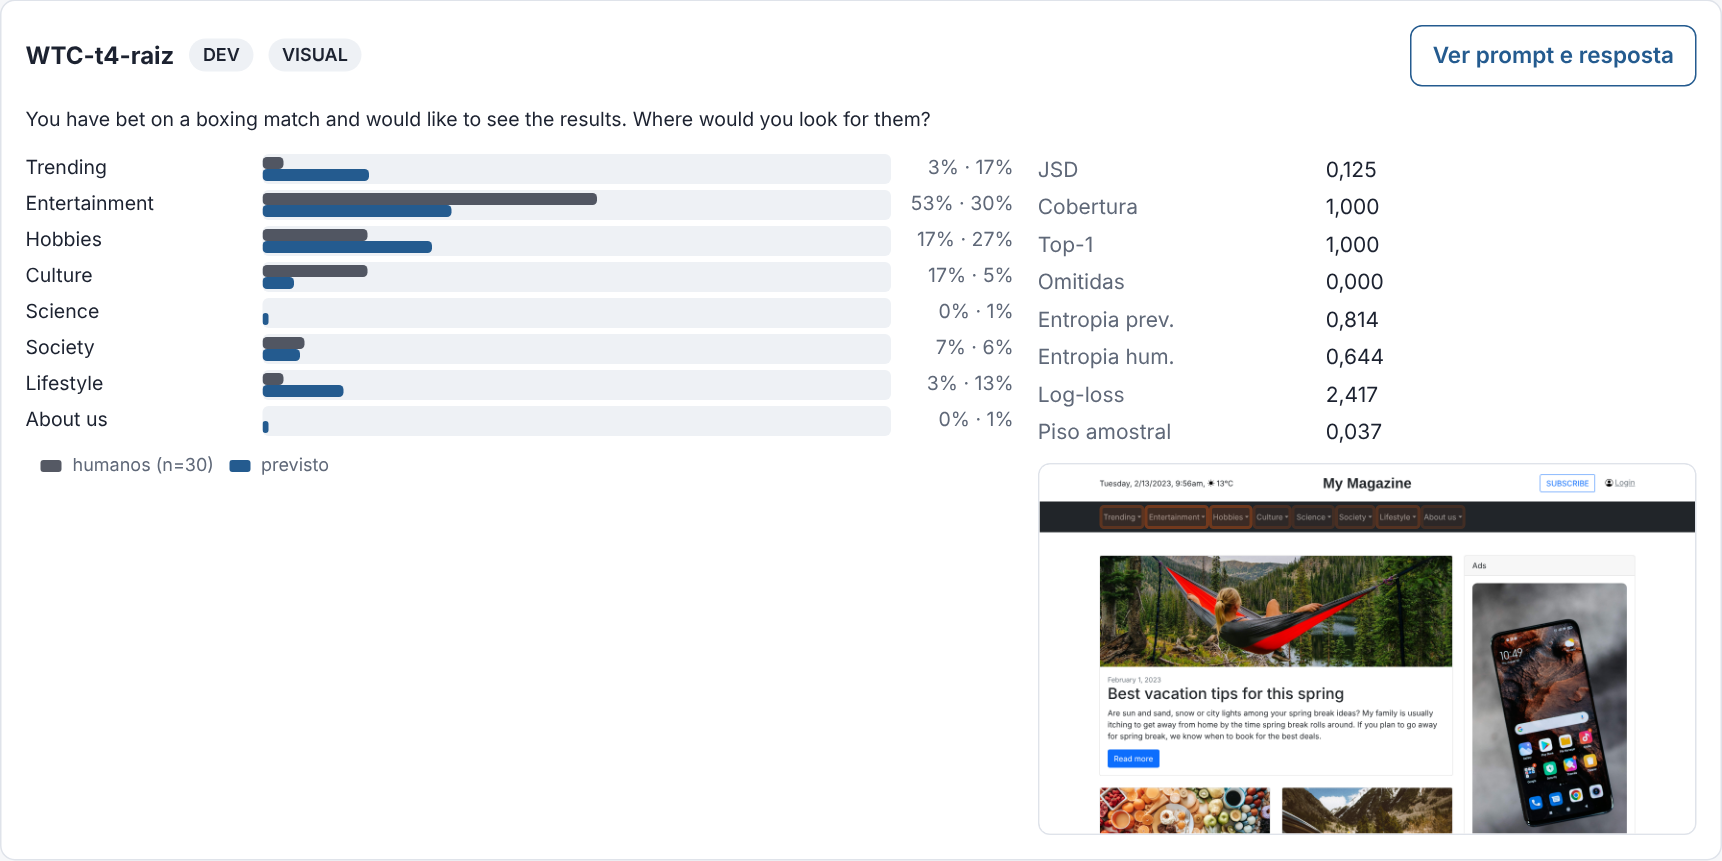
\includegraphics[width=\textwidth]{figuras/painel-previsao-b1cw.png}
\caption{Painel do modo NAV, um estado do piloto (WTC, tarefa 4, B1-CW com Claude Opus~5.5): barras humanas (cinza, $n=30$) e previstas (azul), métricas do estado e tela com as opções destacadas pela probabilidade prevista.}
\label{fig:painel}
\end{figure}

%%%%%%%%%%%%%%%%%%%%%%%%%%%%%%%%%%%%%%
\section{Passo a passo do experimento}
\label{sec:passos}

Esta seção descreve, em ordem, o que é feito em cada etapa e o que cada etapa produz. As etapas 1 a 8 já foram executadas; as demais estão planejadas.

\begin{enumerate}[leftmargin=*,label=\textbf{Passo \arabic*.},itemsep=3pt]
\item \textbf{Fixar os dados.} Baixar o repositório de Kuric et al. \cite{kuric2025dataset} na revisão \code{6cc9130}. \emph{Produz:} uma cópia imutável dos dados e dos protótipos.
\item \textbf{Importar e contar.} Para cada uma das 1.800 execuções, tomar o primeiro clique e reduzi-lo à categoria do primeiro nível; descartar as 4 sem clique; agregar por variante e tarefa. \emph{Produz:} 60 estados com contagens humanas, verificados contra uma recontagem independente.
\item \textbf{Renderizar as telas.} Para WTC, WTCI e WM, abrir o protótipo com relógio congelado, extrair as opções e suas coordenadas e salvar a captura. \emph{Produz:} 3 telas idênticas byte a byte em qualquer importação.
\item \textbf{Dividir.} Tarefas pares em DEV e ímpares em TEST. \emph{Produz:} 30 estados de cada lado.
\item \textbf{Montar as entradas.} Para cada estado, gerar o \code{NavInput} (tarefa, opções e tela) e o \textit{hash} da entrada. \emph{Produz:} entradas auditáveis, sem dados humanos.
\item \textbf{Rodar as referências.} UNIFORM e B0, com $\tau$ do B0 ajustado só no DEV. \emph{Produz:} previsões, métricas e \textit{hashes} congelados; conferência independente em Python.
\item \textbf{Piloto pequeno com LLMs.} B1 e B1-CW, em Claude e GPT-4.1, em 4 estados do DEV, para verificar prompts, respostas, armazenamento, isolamento das entradas e custo real. \emph{Produz:} o relatório da Seção~\ref{sec:piloto}.
\item \textbf{B0 em validação cruzada.} Ajustar $\tau$ em cada metade das tarefas e avaliar na outra (Seção~\ref{sec:resultados}).
\item \textbf{Revisão do método (planejado).} Análise dos resultados preliminares e decisão sobre os pontos em aberto da Seção~\ref{sec:plano}. Ajustes de prompt, se houver, usam só o DEV e geram nova versão.
\item \textbf{Congelar parâmetros e orçamento (planejado).} Registrar versão dos prompts, modelos, esforço, $N$, limiares e semente; estimar o custo a partir dos \textit{tokens} medidos; obter aprovação.
\item \textbf{Rodar as condições B1 uma única vez (planejado).} B1, B1-CW, B1-R, B1-S e B1-CW-S nos dois modelos, em todos os 60 estados (40 entradas distintas), com os parâmetros congelados. Uma rodada de verificação em poucos estados vem antes, para confirmar custo e estabilidade.
\item \textbf{Analisar (planejado).} Diferenças pareadas de H1--H3 nas 10 tarefas, com IC por tarefa e teste exato de troca de sinal; B1 reamostrado para H2; análise por modalidade e variante (H4); casos de omissão; custo por ponto de JSD.
\item \textbf{Piloto institucional (planejado).} Capturar a página inicial das tarefas do IFPB, congelar as previsões e só depois coletar as escolhas de iniciantes (Seção~\ref{sec:ifpb}).
\item \textbf{B2, se justificado (planejado).} Comparar um sistema multiagente com o melhor B1, com orçamento equivalente.
\end{enumerate}

%%%%%%%%%%%%%%%%%%%%%%%%%%%%%%%%%%%%%%
\section{Validação da implementação}
\label{sec:validacao}

\begin{real}
Antes de interpretar qualquer métrica, conferimos se o protótipo mede o que diz medir. A Tabela~\ref{tab:validacao} resume as verificações. Todas foram feitas com dados reais; os \textit{scripts} estão no repositório.
\end{real}

\begin{table}[ht]
\centering
\caption{Verificações da implementação.}
\label{tab:validacao}
\scriptsize
\begin{tabularx}{\textwidth}{@{}p{2.8cm}Yp{3.6cm}@{}}
\toprule
\textbf{O que} & \textbf{Como} & \textbf{Resultado} \\
\midrule
Contagens humanas & Recontagem independente em Python, direto do \code{results.csv} bruto & 60/60 estados iguais; textos das tarefas idênticos \\
Tokenizador e \textit{embeddings} do B0 & 12 textos de referência (acentos, pontuação, CJK) contra \code{tokenizers} e \code{onnxruntime} em Python & \textit{Tokens} idênticos; vetores iguais até $10^{-4}$ \\
Temperatura do B0 & Reajuste independente em Python, mesma grade, 30 estados DEV & $\tau=0{,}060912$ nos dois \\
Distribuições do B0 & Recalculadas em Python & Diferença máxima $6\times10^{-7}$ \\
Métricas & Reimplementação independente; JSD via \code{scipy} (base 2, ao quadrado) & Diferença máxima $\approx10^{-15}$ \\
Reprodutibilidade & Duas execuções do zero (banco, armazenamento e modelo novos) e rodadas repetidas & Mesmo \textit{hash} das entradas e mesmos \textit{hashes} congelados \\
Telas & Comparação byte a byte entre importações & WTC, WTCI e WM idênticas \\
Isolamento das entradas & Teste estrutural de \code{NavInput}; auditoria dos 16 prompts do piloto (só tarefa, uma frase sobre a tela e uma linha por opção; todo número vem da tarefa, dos ids ou das coordenadas) & 16/16 limpos \\
\textit{Cache} e custo & Rodada do piloto repetida & 0 chamadas, 0 \textit{tokens}, mesmo \textit{hash} \\
Testes automatizados & JUnit (19 testes) & Todos passando \\
\bottomrule
\end{tabularx}
\end{table}

\textbf{Problemas encontrados e corrigidos.} A validação encontrou cinco problemas, todos corrigidos antes dos resultados abaixo:
\begin{enumerate}[leftmargin=*,itemsep=0pt]
\item O anúncio animado do protótipo WTCI tornava a tela diferente a cada importação, o que mudava o \textit{hash} da entrada. Corrigido com relógio simulado e congelado.
\item A concordância top-1 contava empates como acerto, e a previsão uniforme ``acertava'' em 100\% dos estados. Corrigido com o desempate aleatório esperado.
\item No Claude, um esquema com o campo \code{thought} disparava recusas por ``extração de raciocínio''. O campo foi renomeado para \code{reason}, e recusas passaram a ser contadas sem interromper a rodada.
\item A ordem das chaves do esquema JSON variava entre execuções da JVM, mudando a chave de \textit{cache} e o \textit{hash} do prompt. Corrigido com mapas ordenados.
\item Rodadas servidas pelo \textit{cache} somavam \textit{tokens} como se tivessem sido gastos. Corrigido para contar só o que foi efetivamente chamado.
\end{enumerate}

%%%%%%%%%%%%%%%%%%%%%%%%%%%%%%%%%%%%%%
\section{Resultados preliminares}
\label{sec:resultados}

\subsection{O que os dados humanos mostram}

\begin{real}
Nos 60 estados, a opção mais escolhida reúne em média 58\% das pessoas, e em 28\% dos estados nenhuma opção chega a 50\%. Há em média 2,6 opções escolhidas por pelo menos 10\% das pessoas (mínimo 1, máximo 4). A entropia normalizada humana média é 0,51 no TEST. O piso amostral da JSD, com 30 pessoas por estado, é 0,027 [0,024; 0,030] no TEST.

A referência humana entre variantes (a distribuição da mesma tarefa nas outras cinco variantes) tem JSD de 0,043 [0,040; 0,047] no TEST: 0,039 nas variantes textuais e 0,048 nas visuais. Ou seja, a distribuição depende muito mais da tarefa e da arquitetura do que da apresentação, e a meta realista de um bom preditor fica entre o piso (0,027) e essa referência (0,043).
\end{real}

\subsection{B0 e UNIFORM}

\begin{real}
A Tabela~\ref{tab:b0} traz os resultados de B0 e UNIFORM. Hashes congelados: UNIFORM \code{7763c445\ldots}, B0 \code{55de6c0f\ldots}. Temperatura do B0 ajustada no DEV: $\tau=0{,}0609$ (JSD média no DEV de 0,281).
\end{real}

\begin{table}[ht]
\centering
\caption{UNIFORM e B0 no \textit{benchmark} (média e IC 95\% por \textit{bootstrap} de tarefas). ↓ menor é melhor; ↑ maior é melhor.}
\label{tab:b0}
\scriptsize
\begin{tabular}{@{}llccccc@{}}
\toprule
\textbf{Grupo} & \textbf{Método} & \textbf{JSD ↓} & \textbf{Cobertura ↑} & \textbf{Top-1 ↑} & \textbf{Omitidas ↓} & \textbf{Entropia prev.} \\
\midrule
TEST, todos & UNIFORM & 0,378 [0,352; 0,402] & 1,000 & 0,133 & 0,00 & 1,000 \\
TEST, todos & B0 & 0,289 [0,217; 0,387] & 0,948 [0,913; 0,975] & 0,433 [0,03; 0,83] & 0,20 & 0,858 \\
TEST, texto & UNIFORM & 0,401 [0,392; 0,413] & 1,000 & 0,133 & 0,00 & 1,000 \\
TEST, texto & B0 & 0,308 [0,215; 0,425] & 0,958 & 0,467 & 0,13 & 0,858 \\
TEST, visual & UNIFORM & 0,354 [0,307; 0,402] & 1,000 & 0,133 & 0,00 & 1,000 \\
TEST, visual & B0 & 0,271 [0,205; 0,357] & 0,938 & 0,400 & 0,27 & 0,858 \\
DEV, todos & B0 & 0,281 [0,202; 0,344] & 0,927 & 0,400 & 0,27 & 0,814 \\
\midrule
\multicolumn{7}{@{}l}{\textit{Log-loss} no TEST: UNIFORM 3,000 bits; B0 2,615 [2,169; 3,205] bits.} \\
\bottomrule
\end{tabular}
\end{table}

\begin{real}
\textbf{Diferença pareada B0 $-$ UNIFORM na JSD:} $-0{,}088$ [$-0{,}172$; $+0{,}029$] no TEST e $-0{,}091$ [$-0{,}149$; $-0{,}020$] no DEV. No TEST, o intervalo cruza zero: com cinco tarefas, ainda não se pode afirmar que o B0 é melhor que o acaso fora do conjunto em que foi ajustado. No DEV a diferença é significativa, mas a temperatura foi ajustada ali.
\end{real}

\begin{real}
\textbf{B0 com validação cruzada, nas 10 tarefas.} Ajustando $\tau$ nas tarefas pares ($\tau=0{,}0609$, o mesmo da rodada) e aplicando às ímpares, e ajustando nas ímpares ($\tau=0{,}0451$) e aplicando às pares, a JSD do B0 nas 10 tarefas é 0,288 [0,239; 0,345], contra 0,375 [0,330; 0,420] do UNIFORM. A diferença pareada é $-0{,}087$ [$-0{,}145$; $-0{,}017$]; o B0 fica abaixo do UNIFORM em 8 das 10 tarefas, com $p=0{,}041$ no teste exato de troca de sinal. Só com as 5 tarefas ímpares, o mesmo teste dá $p=0{,}25$, e nunca poderia ficar abaixo de 0,0625. Ou seja, o efeito do B0 já era o mesmo ($-0{,}088$ só nas ímpares); o que mudou foi a capacidade de detectá-lo. Cálculo em \code{analysis/nav\_b0\_crossfit.py}, sem chamadas a LLMs.
\end{real}

A Figura~\ref{fig:variantes} mostra a JSD por variante. Como o B0 só usa texto, ele prevê a mesma distribuição para as seis variantes de uma tarefa; as diferenças entre variantes vêm só dos humanos.

\begin{figure}[ht]
\centering
\begin{tikzpicture}
\begin{axis}[
  ybar, bar width=9pt, width=0.85\textwidth, height=5.2cm,
  ymin=0, ymax=0.48, ylabel={JSD média (todas as tarefas)},
  symbolic x coords={TP,TC,TO,WTC,WTCI,WM}, xtick=data,
  legend style={at={(0.5,1.03)},anchor=south,legend columns=-1,font=\scriptsize},
  ticklabel style={font=\scriptsize}, label style={font=\scriptsize},
  nodes near coords, nodes near coords style={font=\tiny, /pgf/number format/fixed, /pgf/number format/precision=2},
  extra y ticks={0.027,0.043}, extra y tick labels={,},
  extra y tick style={grid=major, grid style={dashed, gray}, tick label style={font=\tiny}}
]
\addplot[fill=gray!40] coordinates {(TP,0.374) (TC,0.410) (TO,0.419) (WTC,0.345) (WTCI,0.365) (WM,0.336)};
\addplot[fill=blue!45] coordinates {(TP,0.286) (TC,0.307) (TO,0.325) (WTC,0.256) (WTCI,0.288) (WM,0.249)};
\legend{UNIFORM, B0}
\end{axis}
\end{tikzpicture}
\caption{JSD por variante, nos 10 estados de cada uma (DEV e TEST juntos; a temperatura do B0 foi ajustada no DEV). Linhas tracejadas: piso amostral (0,027) e referência humana entre variantes (0,043), ambos no TEST.}
\label{fig:variantes}
\end{figure}

\textbf{Onde o B0 erra.} O B0 segue a semelhança literal entre palavras, não o modelo mental do leitor. Na tarefa 2 (filme de comédia para uma noite com amigos), 26 de 30 pessoas da variante TP escolheram Entertainment, mas o B0 pôs Hobbies em primeiro (0,41). Na tarefa 7 (vida na Idade Média), 17 das 30 pessoas da variante TP escolheram Culture, e o B0 preferiu Lifestyle. Esta análise de erros do B0 foi feita depois de suas previsões estarem congeladas e não alimenta nenhum ajuste. Esses casos são exatamente os que um preditor com conhecimento de mundo deveria resolver.

\subsection{Piloto pequeno com LLMs}
\label{sec:piloto}

\begin{real}
\textbf{Desenho.} Quatro estados do DEV, escolhidos para cobrir os casos: TP-t2 (texto, humanos concentrados), TP-t8 (texto, humanos dispersos), WTC-t4 (visual, \textit{desktop}) e WM-t8 (visual, celular, humanos dispersos). B1 e B1-CW, uma chamada por estado, em Claude Opus~5.5 e GPT-4.1, esforço \code{medium}, prompts \code{nav-1.1}. Nenhum estado do TEST foi enviado a LLMs. A Tabela~\ref{tab:piloto} traz as médias e a Tabela~\ref{tab:pilotoestados}, os estados.
\end{real}

\begin{table}[ht]
\centering
\caption{Piloto: médias nos 4 estados DEV. Custo estimado por preço de tabela (Claude US\$~4/20 e GPT-4.1 US\$~2/8 por milhão de \textit{tokens} de entrada/saída; o preço do GPT-4.1 ainda precisa ser conferido).}
\label{tab:piloto}
\scriptsize
\begin{tabular}{@{}llcccccc@{}}
\toprule
\textbf{Método} & \textbf{Modelo} & \textbf{JSD ↓} & \textbf{Cobertura ↑} & \textbf{Top-1 ↑} & \textbf{Entropia prev.} & \textbf{\textit{Tokens} (ent./saída)} & \textbf{Custo} \\
\midrule
B0 & -- & 0,285 & 0,958 & 0,00 & 0,88 & -- & 0 \\
B1 & Claude Opus 5.5 & 0,131 & 0,942 & 0,25 & 0,69 & 4.612 / 937 & US\$ 0,037 \\
B1-CW & Claude Opus 5.5 & 0,119 & 0,933 & 0,50 & 0,70 & 6.572 / 2.018 & US\$ 0,067 \\
B1 & GPT-4.1 & 0,195 & 0,875 & 0,38 & 0,72 & 2.839 / 964 & US\$ 0,013 \\
B1-CW & GPT-4.1 & 0,248 & 0,725 & 0,50 & 0,54 & 3.695 / 1.693 & US\$ 0,021 \\
\bottomrule
\end{tabular}
\end{table}

\begin{table}[ht]
\centering
\caption{Piloto, por estado: JSD e as três opções mais prováveis previstas. Humanos: as opções com pelo menos 4 escolhas.}
\label{tab:pilotoestados}
\scriptsize
\begin{tabularx}{\textwidth}{@{}p{1.3cm}p{2.9cm}cccccY@{}}
\toprule
\textbf{Estado} & \textbf{Humanos ($n=30$)} & \textbf{B0} & \textbf{B1 Cl.} & \textbf{B1-CW Cl.} & \textbf{B1 GPT} & \textbf{B1-CW GPT} & \textbf{Destaque} \\
\midrule
TP-t2 & Entertainment 26 & 0,416 & 0,082 & 0,075 & 0,187 & 0,173 & B0 erra a moda (Hobbies); LLMs acertam. \\
TP-t8 & Lifestyle 12, Hobbies 7, Entertainment 5, Science 4 & 0,218 & 0,149 & 0,160 & 0,181 & 0,198 & Claude põe Science em 1º (0,40): viés de ``especialista''. \\
WTC-t4 & Entertainment 16, Hobbies 5, Culture 5 & 0,285 & 0,144 & 0,125 & 0,243 & 0,359 & GPT põe Trending em 1º; B1-CW concentra mais. \\
WM-t8 & Hobbies 8, Entertainment 7, Science 7, Lifestyle 5 & 0,219 & 0,148 & 0,118 & 0,170 & 0,261 & Distribuição humana muito dispersa. \\
\bottomrule
\end{tabularx}
\end{table}

\begin{real}
\textbf{O que o piloto indica} (quatro estados; não é teste de hipótese):
\begin{itemize}[leftmargin=*,itemsep=0pt]
\item O B1, nos dois modelos, e o B1-CW do Claude ficaram abaixo do B0 em JSD nos quatro estados. O B1-CW do GPT-4.1 ficou acima do B0 em dois (WTC-t4 e WM-t8).
\item O efeito de Q1--Q3 mudou de direção conforme o modelo. No Claude, o B1-CW reduziu a JSD em 3 de 4 estados (0,131 $\to$ 0,119). No GPT-4.1, aumentou em 3 de 4 (0,195 $\to$ 0,248), reduzindo a entropia (0,72 $\to$ 0,54) e a cobertura (0,875 $\to$ 0,725). As perguntas deixaram o GPT mais concentrado. É o tipo de interação modelo $\times$ condição que H1 precisa testar com todos os estados.
\item Armazenamento e auditoria funcionaram: 16 previsões, 0 respostas inválidas, 0 recusas, prompts limpos.
\item Custo do piloto: cerca de US\$~0,14 estimado (16 chamadas). Os testes de funcionamento anteriores (5 estados, incluindo amostragem) custaram cerca de US\$~0,60 estimados. O custo real é o do painel de faturamento de cada fornecedor.
\end{itemize}

\textbf{Amostragem (teste de funcionamento).} Em testes de funcionamento do B1-S com poucas amostras (5 estados DEV; $N=3$ no Claude e $N=5$ no GPT-4.1), as duas LLMs deram quase sempre a mesma escolha para o mesmo estado: entropia prevista de 0,00 (Claude) e 0,05 (GPT-4.1), com JSD de 0,50 e 0,47. É a subdispersão relatada em \cite{kuric2026wwgc}. Com $N$ tão pequeno, isso é só um indício; a medida está prevista no experimento completo.
\end{real}

\begin{figure}[ht]
\centering
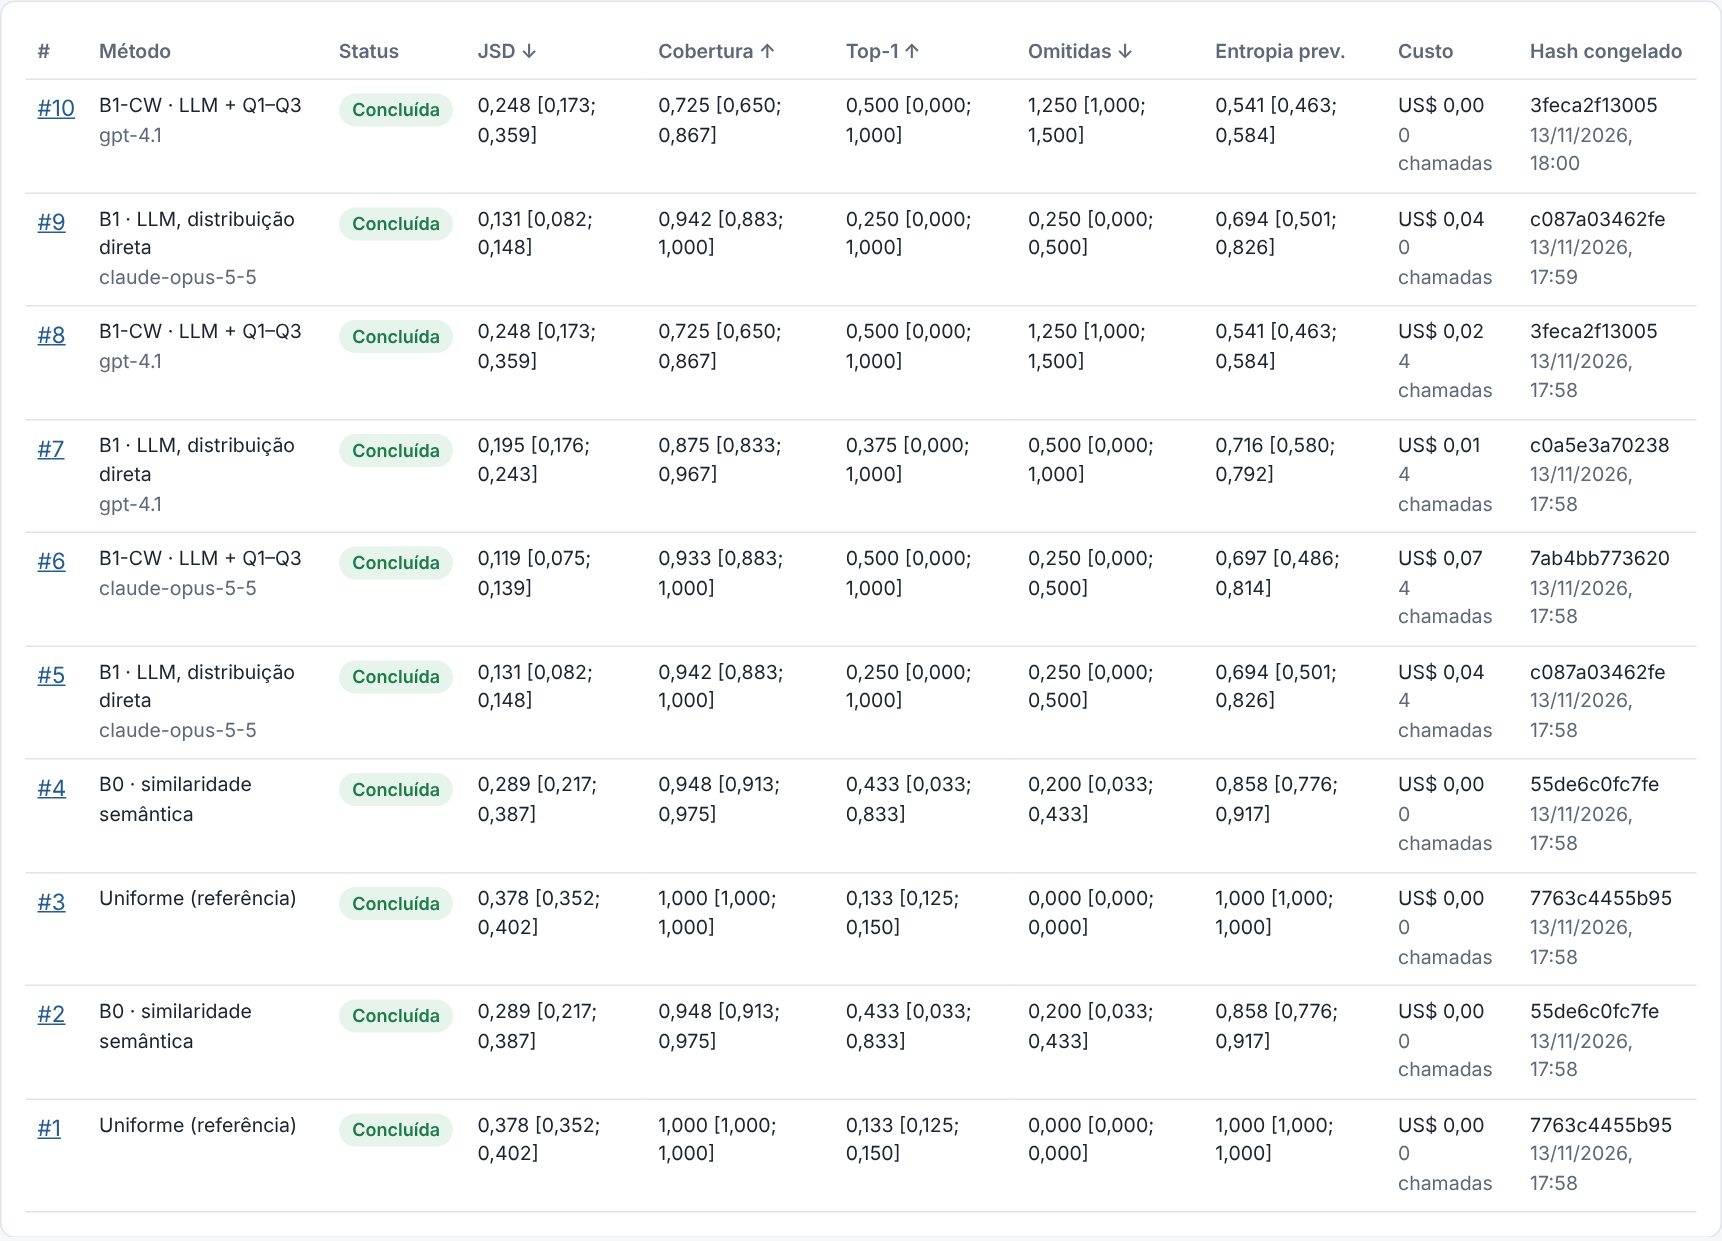
\includegraphics[width=\textwidth]{figuras/painel-comparacao.png}
\caption{Painel: comparação das rodadas no \textit{benchmark} (métricas, custo e \textit{hash} congelado de cada rodada).}
\label{fig:comparacao}
\end{figure}

%%%%%%%%%%%%%%%%%%%%%%%%%%%%%%%%%%%%%%
\section{Piloto no portal do IFPB}
\label{sec:ifpb}

\begin{planejado}
O portal do IFPB é usado como estudo piloto prospectivo: as previsões são geradas e congeladas \emph{antes} de qualquer coleta com pessoas. Não é um teste cego do método, porque o pesquisador conhece o portal; é uma verificação de que o fluxo funciona num caso real e em português.
\end{planejado}

\textbf{Tarefa inicial.} Localizar o Edital nº 01/2026 de credenciamento do Banco de Especialistas do Polo de Inovação, a partir da página do Polo. A tarefa já está cadastrada no protótipo. Na fase de coleta, outras tarefas típicas de ingressantes serão acrescentadas (por exemplo, emitir uma declaração de matrícula ou achar o calendário acadêmico).

\textbf{Passos.}
\begin{enumerate}[leftmargin=*,itemsep=1pt]
\item Capturar a página inicial de cada tarefa com a captura independente (Figura~\ref{fig:captura}), na instância implantada do protótipo (o portal não é acessível a partir do ambiente de desenvolvimento).
\item Mapear, antes da análise, as opções que levam ao destino ($V(s)$), para calcular o risco de desvio.
\item Rodar UNIFORM, B0 e as condições B1 com os parâmetros congelados. Para o B0 em português, trocar o modelo de \textit{embeddings} por uma versão multilíngue (por exemplo, paraphrase-multilingual-MiniLM-L12-v2, como em \cite{jin2026scent}), ajustada sem dados do IFPB.
\item Registrar os \textit{hashes} congelados e exportar as previsões.
\item Só depois, com aprovação do comitê de ética, coletar primeiros cliques de ingressantes (teste de primeiro clique ou \textit{tree testing}, com perfil de iniciante declarado) e calcular as métricas.
\end{enumerate}

\begin{figure}[ht]
\centering

\includegraphics[width=0.75\textwidth]{figuras/captura-portal-ficticio.png}
\caption{Captura independente executada no portal fictício do protótipo, que reproduz a estrutura do caso do IFPB: só a página inicial, sem seguir a rota; o estado gerado tem 11 opções visíveis e nenhum dado humano.}
\label{fig:captura}
\end{figure}

\begin{real}
A captura independente já foi executada no portal fictício que acompanha o protótipo e reproduz a estrutura do caso do IFPB (Figura~\ref{fig:captura}). O estado gerado tem 11 opções visíveis (``Núcleo de Inovação'', ``Editais e Concursos'' etc.), partição PILOTO e nenhum dado humano.
\end{real}

\textbf{Cuidados éticos.} A navegação automatizada só faz requisições GET em páginas públicas, sem cadastro, sem formulários e com intervalo entre ações. A coleta com pessoas só começa após aprovação do CEP \cite{cns2016res510}, com consentimento, anonimização e tratamento conforme a LGPD \cite{brasil2018lgpd}.

%%%%%%%%%%%%%%%%%%%%%%%%%%%%%%%%%%%%%%
\section{Plano do experimento completo}
\label{sec:plano}

\begin{planejado}
\textbf{Escopo.} As cinco condições com LLM (B1, B1-CW, B1-R, B1-S e B1-CW-S) em Claude Opus~5.5 e GPT-4.1, uma única vez, nos 60 estados, depois de uma verificação curta em poucos estados. Como as três variantes textuais dão ao modelo a mesma entrada, há 40 entradas distintas (10 textuais e 30 visuais); estados com a mesma entrada recebem a mesma previsão, servida pelo \textit{cache}.

\textbf{Custo estimado.} A partir dos \textit{tokens} medidos no piloto e nos testes de funcionamento: cerca de US\$~29 no Claude e US\$~9 no GPT-4.1 para as cinco condições em todos os estados, dominados pelas condições amostradas ($N=30$, cerca de 1.200 chamadas por condição e modelo). O controle B1-R acrescenta cerca de US\$~1 no total (40 chamadas por modelo). São estimativas, não orçamentos: o valor real será medido e o experimento só roda com aprovação.

\textbf{Pontos a decidir antes de rodar:}
\begin{enumerate}[leftmargin=*,itemsep=0pt]
\item \textit{Decidido:} avaliar as hipóteses nas 10 tarefas, com $\tau$ do B0 em validação cruzada, e incluir o controle B1-R.
\item Manter as três variantes textuais na média (a dependência já é tratada pelo \textit{bootstrap} por tarefa) e relatar à parte a variação humana entre elas.
\item Manter o B1-S como pré-registrado e relatar o colapso, se confirmado, como resultado. Variar a \textit{persona} seria uma nova condição (B1-P), para depois.
\item Confirmar o preço vigente do GPT-4.1 e decidir se o GPT-5.2 entra como terceiro modelo.
\item Fixar a versão dos prompts (\code{nav-1.1} ou uma revisão feita só no DEV).
\end{enumerate}
\end{planejado}

%%%%%%%%%%%%%%%%%%%%%%%%%%%%%%%%%%%%%%
\section{Ameaças à validade}
\label{sec:ameacas}

\textbf{Validade interna.}
\begin{itemize}[leftmargin=*,itemsep=0pt]
\item \textit{Vazamento de respostas.} Mitigado pelo isolamento estrutural das entradas, pela captura independente e pela auditoria dos prompts.
\item \textit{Ajuste no conjunto de avaliação.} A temperatura do B0 é ajustada em validação cruzada, e nenhum estado é avaliado com um $\tau$ ajustado nele. Os prompts das condições com LLM foram escritos antes de qualquer rodada nos dados e só foram testados em 4 estados das tarefas pares; uma eventual revisão gera nova versão e é relatada. Cada condição roda uma única vez.
\item \textit{Deliberação como confusão.} Pedir Q1--Q3 também faz o modelo escrever mais. O controle B1-R separa os dois efeitos.
\item \textit{Contaminação do modelo.} O repositório do \textit{benchmark} é público desde 2025, e um LLM pode ter visto os dados. O risco é menor porque o modelo nunca recebe os rótulos da árvore completa nem as contagens, e será medido comparando o desempenho com o do piloto prospectivo no IFPB, cujos dados ainda não existem.
\item \textit{Não determinismo.} As respostas das APIs variam entre chamadas. Todas as respostas ficam armazenadas, e a análise usa as respostas registradas; a variação entre chamadas é medida no B1-S.
\end{itemize}

\textbf{Validade de construto.}
\begin{itemize}[leftmargin=*,itemsep=0pt]
\item O primeiro clique numa categoria do primeiro nível é só o início da navegação. Erros mais profundos e recuperações não são previstos nesta fase.
\item Os participantes do \textit{benchmark} são adultos recrutados \textit{online} e não necessariamente iniciantes no sentido de ingressantes de uma instituição. O \textit{site} é fictício e não é familiar a ninguém, o que aproxima a situação de um primeiro acesso.
\item A JSD resume a distância entre distribuições, mas não diz se o erro está nas opções populares ou nas raras; por isso cobertura e omissões são relatadas junto.
\end{itemize}

\textbf{Validade de conclusão.} Mesmo com 10 tarefas, a amostra de tarefas é pequena e os intervalos por \textit{bootstrap} são largos; com 10 grupos o \textit{bootstrap} ainda pode subestimar a incerteza, por isso o teste exato de troca de sinal é exigido junto. Diferenças pequenas não serão detectáveis; isso será declarado, e os tamanhos de efeito serão relatados com intervalo. O B1-S tem ruído amostral próprio, tratado pela comparação com o B1 reamostrado.

\textbf{Validade externa.} Um \textit{site} de revista em inglês não é um portal institucional em português. O piloto no IFPB testa justamente essa transferência, mas com poucas tarefas. Resultados com dois modelos de 2026 podem não valer para versões futuras.

%%%%%%%%%%%%%%%%%%%%%%%%%%%%%%%%%%%%%%
\section{Cronograma}
\label{sec:cronograma}

\begin{figure}[ht]
\centering
\begin{ganttchart}[
  hgrid, vgrid, x unit=0.62cm, y unit chart=0.5cm,
  title label font=\scriptsize, bar label font=\scriptsize, group label font=\scriptsize\bfseries,
  bar/.append style={fill=blue!35}, group/.append style={fill=gray!60},
  milestone label font=\scriptsize\itshape
]{1}{18}
\gantttitle{2026}{2}\gantttitle{2027}{12}\gantttitle{2028}{4}\\
\gantttitlelist{11,12,1,2,3,4,5,6,7,8,9,10,11,12,1,2,3,4}{1}\\
\ganttgroup{Marco 2: método e \textit{benchmark}}{1}{4}\\
\ganttbar[bar/.append style={fill=green!50}]{Protótipo NAV, B0, piloto (feito)}{1}{1}\\
\ganttbar{Revisão do método e orçamento}{2}{2}\\
\ganttbar{B1 completo: DEV e TEST}{2}{4}\\
\ganttmilestone{Artigo do \textit{benchmark}}{5}\\
\ganttgroup{Marco 3: portal institucional}{4}{11}\\
\ganttbar{Submissão ao CEP}{4}{6}\\
\ganttbar{Capturas e previsões congeladas}{6}{7}\\
\ganttbar{Coleta com ingressantes}{8}{10}\\
\ganttbar{Análise prospectiva}{10}{11}\\
\ganttgroup{Marco 4: extensões}{11}{16}\\
\ganttbar{B2 multiagente (se justificado)}{11}{14}\\
\ganttbar{Escrita da dissertação}{13}{17}\\
\ganttmilestone{Defesa}{18}
\end{ganttchart}
\caption{Cronograma proposto (meses). A barra verde já foi concluída.}
\label{fig:gantt}
\end{figure}

%%%%%%%%%%%%%%%%%%%%%%%%%%%%%%%%%%%%%%
\section{Considerações finais}

O \proj{} trata a previsão de navegação de iniciantes como um problema de distribuição, mensurável contra escolhas humanas, e propõe medir de forma controlada se princípios do percurso cognitivo e estratégias de amostragem tornam as previsões de LLMs mais fiéis. A infraestrutura para isso está construída e foi conferida de forma independente. A \textit{baseline} semântica e a referência uniforme estão medidas, e a meta realista ficou clara: um bom preditor deveria chegar perto de 0,03--0,04 de JSD, onde está a variação natural entre amostras humanas, enquanto o B0 está em 0,29 e o acaso em 0,38. Com $\tau$ em validação cruzada e as 10 tarefas, o B0 fica abaixo do acaso de forma detectável ($-0{,}087$, $p=0{,}041$). O piloto pequeno mostrou que o pipeline com LLMs funciona, que o custo por estado é baixo e que o efeito dos princípios cognitivos pode depender do modelo; o controle B1-R vai dizer se esse efeito vem das perguntas do percurso cognitivo ou apenas de deliberar mais. O próximo passo é o experimento completo, com parâmetros congelados e orçamento aprovado; depois, o piloto prospectivo no portal do IFPB.

\bibliographystyle{sbc}
\bibliography{references}

%%%%%%%%%%%%%%%%%%%%%%%%%%%%%%%%%%%%%%
\appendix

\section{Prompts (versão \code{nav-1.1})}
\label{ap:prompts}

\textbf{B1 (distribuição declarada), prompt do sistema:}
\begin{lstlisting}
You model how real people navigate websites. You will receive a task and the options visible on one screen.
Estimate the distribution of FIRST choices that a population of novices would make: a first-time visitor who has never used this website and does not know how its content is organized.
Do not tell which option is correct. Estimate what such people would actually click, including plausible
mistakes and minority choices. Give a probability to every option id; the probabilities must sum to 1.
\end{lstlisting}

\textbf{B1-CW: o mesmo texto, acrescido de:}
\begin{lstlisting}
Before estimating, apply the cognitive walkthrough questions that make sense before the first action,
to every option, from the novice's point of view:
Q1 (goal): would a novice with this task plausibly decide to look under this option?
Q2 (visibility): is the option noticeable on this screen, considering position, size and contrast?
Q3 (association): does the option's label connect to the task in the novice's own vocabulary?
Q4 (feedback after the action) does not apply here, because the result of the click is not visible yet.
Base the distribution on these answers.
\end{lstlisting}

\textbf{B1-R (controle): o texto do B1, acrescido de:}
\begin{lstlisting}
Before estimating, write a brief analysis of every option: in one short sentence, what a visitor would
expect to find under it and how it relates to the task.
Base the distribution on this analysis.
\end{lstlisting}

\textbf{B1-S (participante simulado), prompt do sistema:}
\begin{lstlisting}
You are a participant in a usability study: a first-time visitor who has never used this website and does not know how its content is organized.
You will receive a task and the options visible on the screen. Choose the option you would click first,
as this participant would, not as an expert. There are no right or wrong answers.
In "reason", say in one short sentence why this participant would click that option.
\end{lstlisting}

\textbf{B1-CW-S: o mesmo texto, acrescido de:}
\begin{lstlisting}
Before choosing, think briefly, as this participant, about each option: would I look here for this task (Q1)?
Do I notice it on the screen (Q2)? Does its label match the words I have in mind (Q3)? Then choose.
\end{lstlisting}

\textbf{Mensagem do usuário (exemplo real do piloto, WTC-t4; a imagem da tela segue junto):}
\begin{lstlisting}
Task: You have bet on a boxing match and would like to see the results. Where would you look for them?

The image shows the screen as the participant sees it before the first click (1366x768 pixels).
Options (id: label @ x,y,width,height):
- 0: Trending @ 125,85,95,48
- 1: Entertainment @ 220,85,133,48
- 2: Hobbies @ 353,85,91,48
- 3: Culture @ 444,85,83,48
- 4: Science @ 527,85,89,48
- 5: Society @ 616,85,85,48
- 6: Lifestyle @ 701,85,92,48
- 7: About us @ 793,85,96,48
\end{lstlisting}

\textbf{Esquemas de resposta.} B1: \code{\{distribution: [\{optionId, probability\}], rationale\}}. B1-CW: \code{\{walkthrough: [\{optionId, q1, q2, q3\}], distribution, rationale\}}, com \code{q1..q3} em \{yes, partly, no\}. B1-R: \code{\{analysis: [\{optionId, note\}], distribution, rationale\}}. B1-S: \code{\{reason, choice\}}. B1-CW-S: \code{\{walkthrough, choice\}}. Em todos, \code{optionId} e \code{choice} são restritos aos identificadores das opções.

\section{Como reproduzir}
\label{ap:repro}

\begin{lstlisting}
# 1. Backend e banco (PostgreSQL 16), sem chaves de API para B0/UNIFORM
cd backend && ./gradlew bootJar
java -jar build/libs/aicogwalk-backend-0.1.0.jar        # porta 8080

# 2. Importar o benchmark (revisão fixada) e rodar as referências
curl -X POST localhost:8080/api/nav/datasets/kuric2025
curl -X POST localhost:8080/api/nav/datasets/1/runs -H 'Content-Type: application/json' -d '{"method":"UNIFORM"}'
curl -X POST localhost:8080/api/nav/datasets/1/runs -H 'Content-Type: application/json' -d '{"method":"B0"}'

# 3. Piloto (requer ANTHROPIC_API_KEY e OPENAI_API_KEY)
curl -X POST localhost:8080/api/nav/datasets/1/runs -H 'Content-Type: application/json' \
  -d '{"method":"B1_CW","model":"gpt-4.1","stateKeys":["TP-t2-raiz","TP-t8-raiz","WTC-t4-raiz","WM-t8-raiz"]}'

# 4. Exportar e conferir em Python
curl localhost:8080/api/nav/runs/2/export.json > b0.json
python3 analysis/verify_b0_metrics.py <dir do modelo> b0.json uniform.json
python3 analysis/nav_kuric_analysis.py uniform.json b0.json
python3 analysis/nav_b0_crossfit.py b0.json
\end{lstlisting}

Os \textit{hashes} esperados para a revisão \code{6cc9130} e os prompts \code{nav-1.1}: UNIFORM \code{7763c4455b95e91d\ldots}, B0 \code{55de6c0fc7fe4083\ldots}. As exportações das rodadas de 13/11/2026 estão em \code{analysis/resultados-2026-11-13/}.

\end{document}
